\documentclass{article}
\usepackage{graphicx}
\title{Project Report CS422}
\author{Sanjana Garg}

\date{}

\begin{document}
\maketitle

\section{Introduction}
Many algorithms have been proposed for improving the performance of L1 and L2 caches but improving the performance of last level cache is equally important since a miss in the last level cache increases the latency of memory operation by many folds. Therefore, it is important to improve the cache hit rate in last-level cache especially for memory intensive applications. But if the working set of an application(the set of most frequently accessed memory locations) is greater than even the size of the last level cache, it can result in a very poor cache performance. Some lines in the working set may get evicted before their use comes. Therefore, it is necessary to maintain a portion of the working set in the cache so that atleast some lines recieve a hit. This particula scenario where the working set is greater than the cache size is termed as thrashing. The algorithms implemented in the project also have the advantage of not having a huge storage overhead.

\section{Methodology}
In the project I have divided the cache policies into two phases: insertion phase and the replacement phase. Insertion policy is required whenever their is a cache miss while replacement policy is needed whenever a victim needs to be chosen to evict from the cache. The three approaches are:
\subsection{Least Recently Used}
This is the traditional LRU approach. In this approach whenever a cache line is accessed it is assigned the status of  most recent. For replacement policy the least recently used cache line is selected and the replaced entry is placed at the most recent position.

\subsection{LRU  Insertion Policy (LIP)}
This is a slight modification of LRU in insertion policy. In this algorithm on a miss the the new cache line is inserted at the least recently used position instead of the most recently used. This way some of the lines are retained from the working set. The victim selection policy is the same as for LRU.

\subsection{Bimodal LIP}
Since using only LIP might perform very badly in programs having affinity for LRU. This algorithm combines the two by placing some incoming lines in MRU while some others at LRU. The probability for placing at MRU is kept low. The threshold is called the bimodal throttling parameter.

\subsection{Random Replacement}
This algorithm keeps the insertion policy the same as LRU but modifies the replacement policy. The cache line to be evicted is selected at random from the set.

\subsection{Cache Configuration}
\begin{itemize}
\item  L1: 32 KB 8-way
\item L2: 256 KB 8-way
\item  L3: 2 MB 16-way 
  \end{itemize}

  \section{Results}
  The reduction in MPKI is plotted in the following histogram. Results were also taken for bzip and perlbench but due to very poor performance they have not been show.
  \begin{figure}[h!]
    \centering
    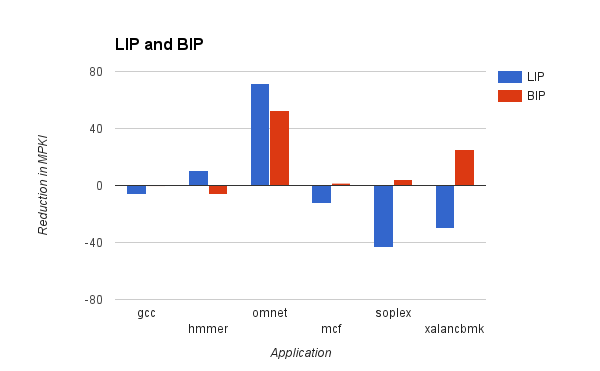
\includegraphics[width=1\textwidth]{image.png}
    \end{figure}
\section{Conclusion}
\begin{itemize}
\item LRU works very well or moderately well for applications with less intensive workloads like gcc and perl.
\item LIP in general alone does not give very good results possibly due to early eviction of cache lines.
  \item BIP performs very well on almost all applications with giving positive results for memory intensive applications. The threshold parameter used for BIP is 0.7.
  \end{itemize}
  \section{Bibliography}
  \begin{itemize}
  \item M. K. Qureshi et al. Adaptive Insertion Policies for High Performance Caching. In Proceedings of the 34th International Symposium on Computer Architecture, pages 381–391, June 2007.
    \item A. Jaleel et al. High Performance Cache Replacement using Re-reference Interval Prediction (RRIP). In Proceedings of the 37th International Symposium on Computer Architecture, pages 60–71, June 2010.
    \end{itemize}
\end{document}
